\documentclass[a4paper]{article}

% import packages
\usepackage{siunitx}
\usepackage[margin=2cm]{geometry}
\usepackage[index]{cuisine}
\usepackage{tocloft}

% main document
\begin{document}

% table of contents
\renewcommand{\contentsname}{\hfill\bfseries\Large Table of Contents\hfill}\renewcommand{\cftaftertoctitle}{\hfill} % change ToC title and center
\tableofcontents % create ToC
\newpage % page break after ToC

% hide section numbers
\renewcommand{\thesection}{}
\renewcommand{\thesubsection}{\arabic{section}.\arabic{subsection}}
\makeatletter
\def\@seccntformat#1{\csname #1ignore\expandafter\endcsname\csname the#1\endcsname\quad}
\let\sectionignore\@gobbletwo
\let\latex@numberline\numberline
\def\numberline#1{\if\relax#1\relax\else\latex@numberline{#1}\fi}
\makeatother

% pressure cooker recipes
\section{Pressure Cooker Recipes}
Some stuff about pressure cooker recipes (maybe a photo).
\begin{recipe}{Pressure Cooker Buffalo Chicken}{4 Portions}{10 Minutes}

\ingredient[2]{lbs}{Chicken}
\ingredient[\fr{2}{3}]{Cup}{Frank's Red Hot}
\ingredient[\fr{1}{3}]{Cup}{Water}
\ingredient[1]{Tbsp}{Butter}
Put all ingredients into the pressure cooker.\\~\\~\\~\\~\\

\newstep
Once the pressure has built, cook for 4 additional minutes on medium.\\~\\

\newstep
Once cooking is finished, turn off the heat and allow the pressure cooker to cool until the pressure is released. Once cool, shred the chicken.

\end{recipe}

\begin{center}
~\\~\\
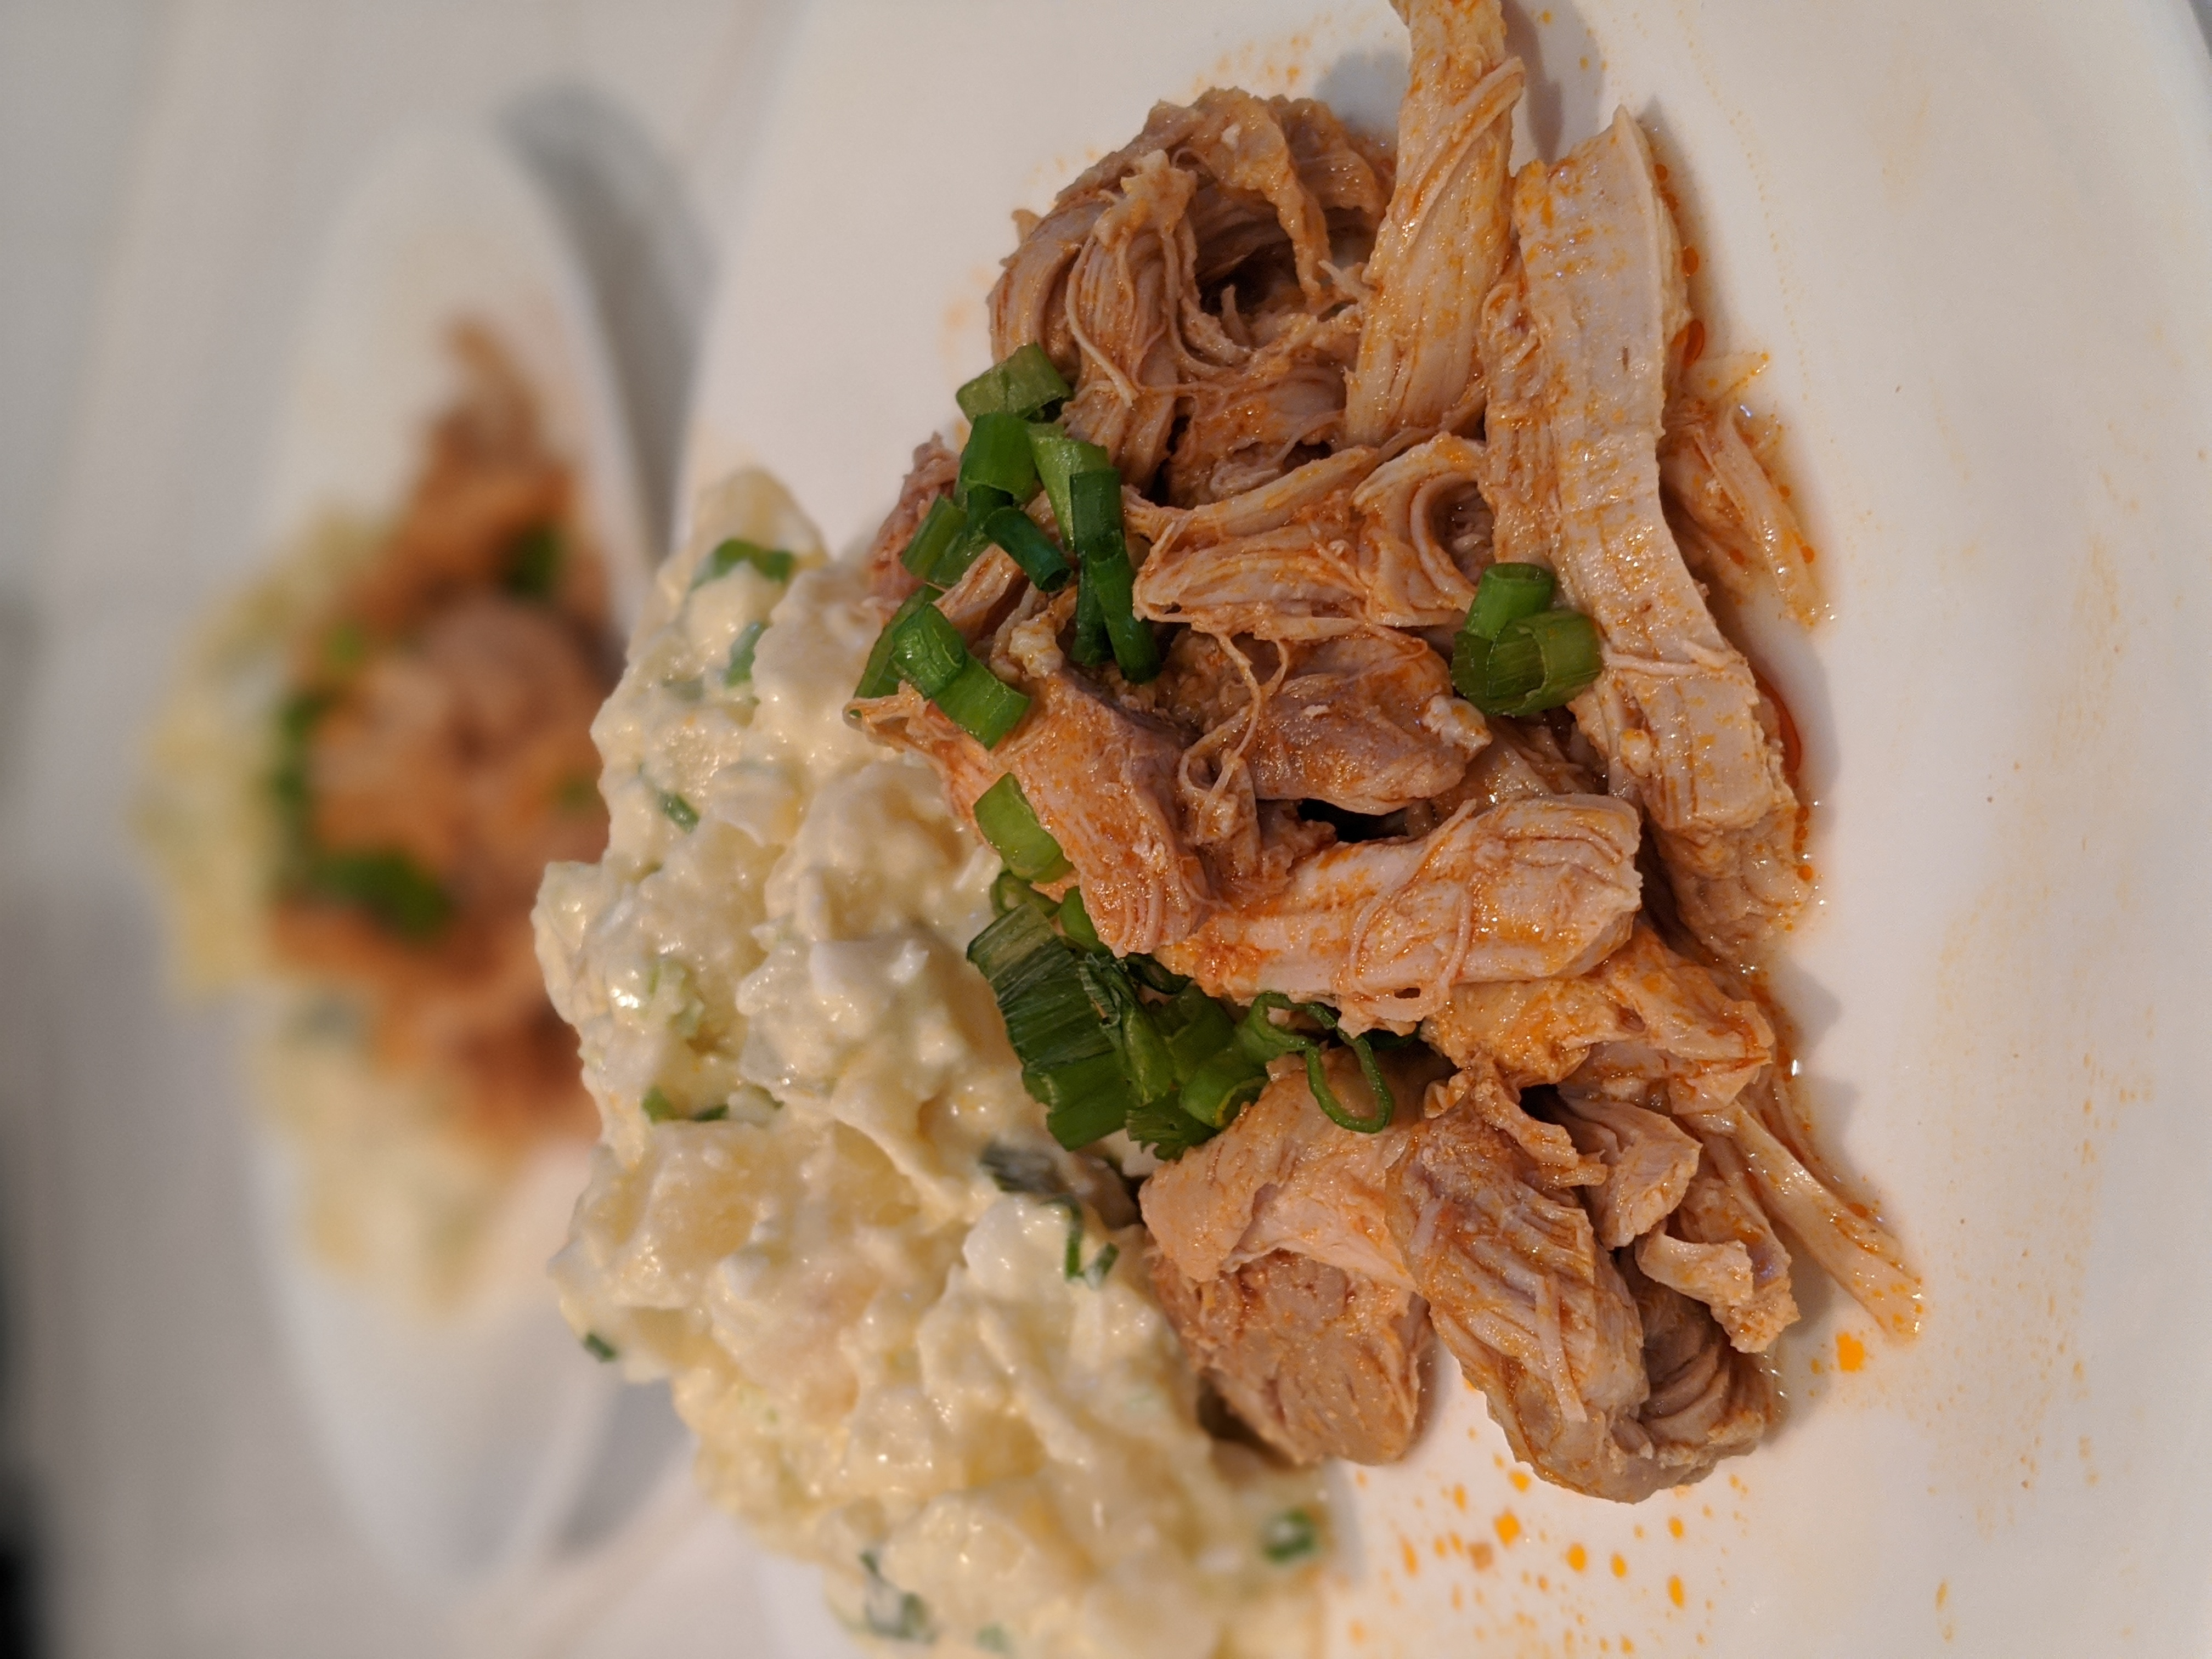
\includegraphics[width=4in,angle=270]{buffalo_chicken_pressure_cooker.jpg}
\end{center}

\end{document}